\chapter{Task \#40: Subways II}


\section{Introduction}


The objective of this data task was to extract node and edge lists from the raw data of subway networks across multiple cities worldwide. To achieve this, three types of scripts were developed, depending on the available information:

\begin{enumerate}
    \item When the topology for a given year was provided as an adjacency matrix, it was used as the primary source to determine the edges.
    \item In the absence of an adjacency matrix, the adjacency list for each year was utilized.
    \item If neither format was available (as was the case for the Chicago subway), edges were inferred from the ``lines'' data.
\end{enumerate}

In instances where specific information was missing from the raw files, the corresponding entries were filled with the placeholder ``unknown'' to preserve the network structure and avoid the removal of any nodes or edges. Data were only removed in cases where there was no correspondence between stations in the files used to infer edges/node IDs and those used to define the nodes.  

The line associated with each edge in the edge list was inferred from the ``line'' files, where available, or from station information files when such data were absent. Mismatches between station names in the node and edge files were resolved using a function that performs a fuzzy string match, accepting matches with at least 70\% character similarity to account for differences in case or whitespace. Node metadata, including latitude, longitude, and year, were extracted from the ``positions-years'' files.  
The resulting node and edge lists were subsequently organized into the folder ``nodes\_edges''.

Having constructed the node and edge lists for the subway networks, we next perform a basic network analysis to characterize their structural properties.



 
\newpage
\section{Basic network analysis}
To understand the structural properties of the network, we analyze the distributions of node degrees and betweenness centrality, which provide insights into node connectivity and their roles in facilitating information flow.
\begin{figure}[hbtp]
    \centering
    \begin{minipage}{0.48\linewidth}
        \centering
        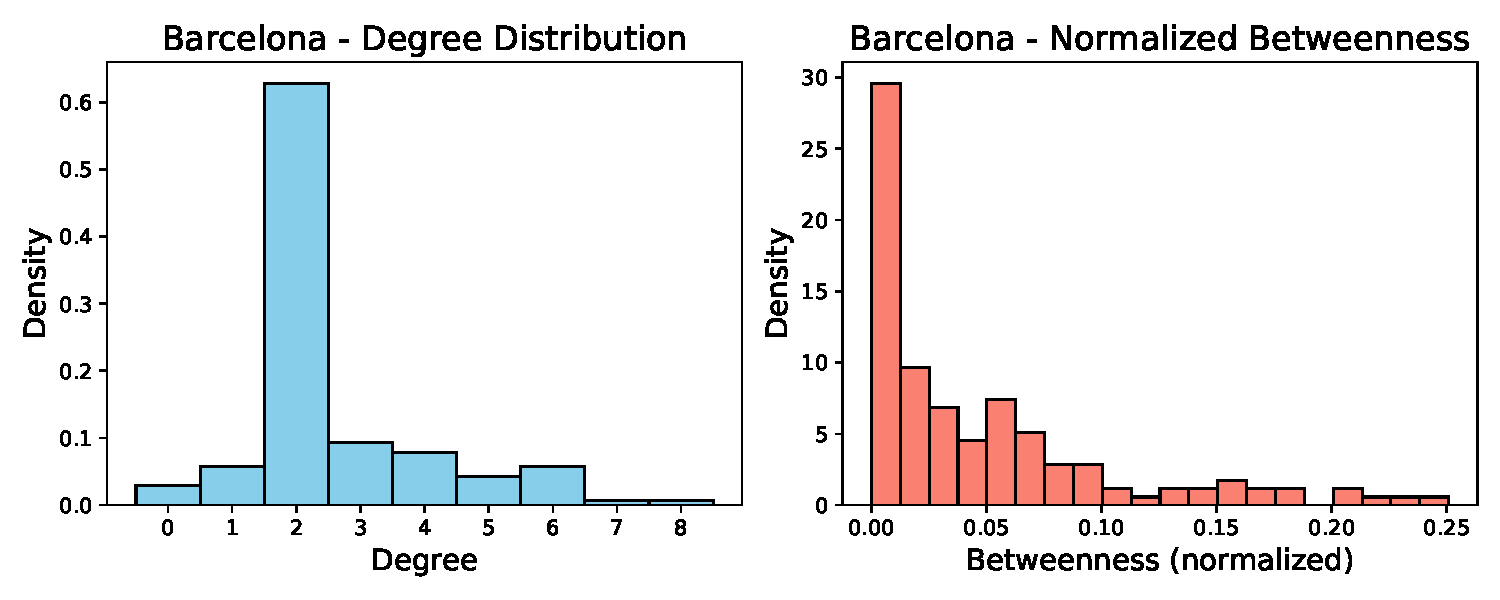
\includegraphics[width=\linewidth]{task40_plots/deg_bet_Barcelona.pdf}
        \end{minipage}%
    \hfill
    \begin{minipage}{0.48\linewidth}
        \centering
        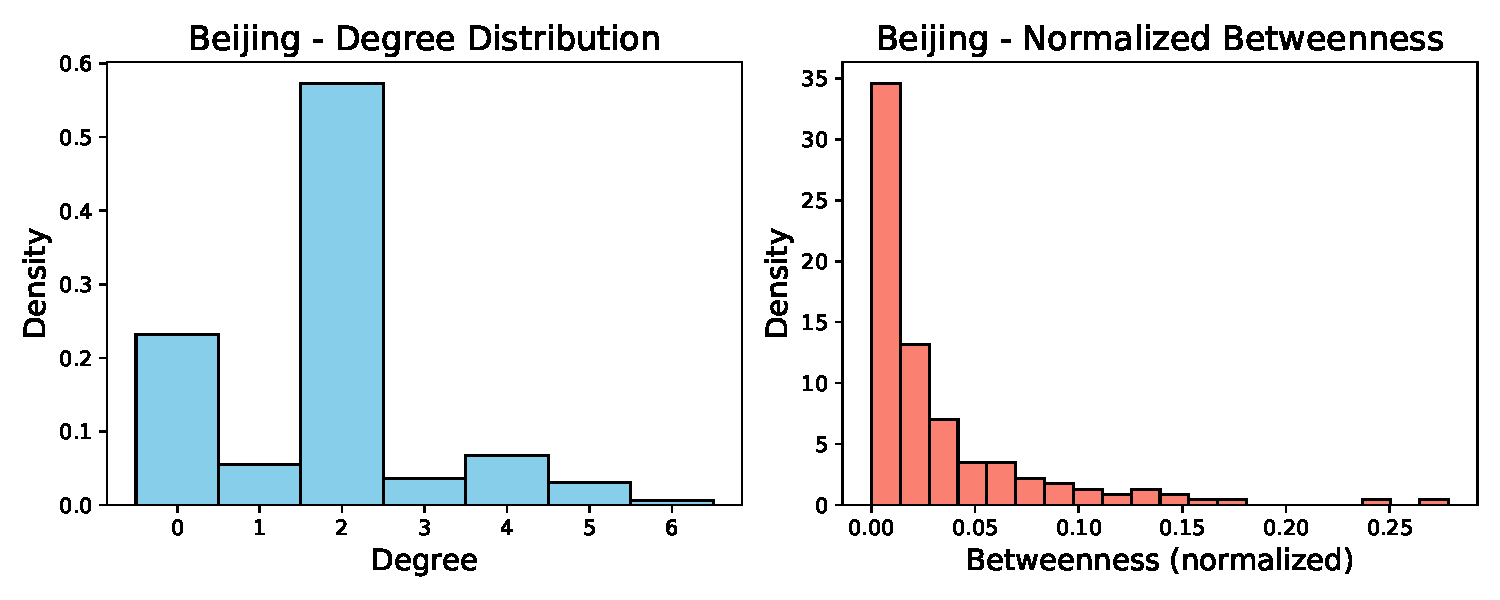
\includegraphics[width=\linewidth]{task40_plots/deg_bet_Beijing.pdf}
    \end{minipage}
\end{figure}

\begin{figure}[hbtp]
    \centering
    \begin{minipage}{0.48\linewidth}
        \centering
        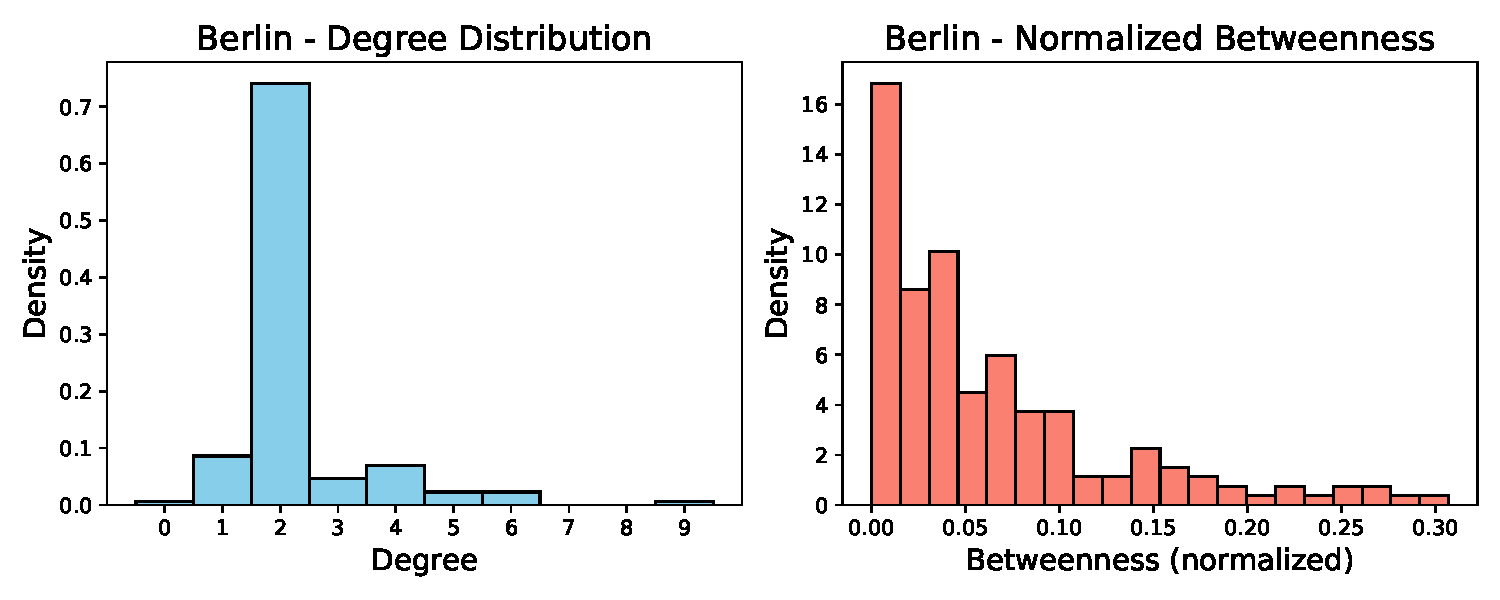
\includegraphics[width=\linewidth]{task40_plots/deg_bet_Berlin.pdf}
        \end{minipage}%
    \hfill
    \begin{minipage}{0.48\linewidth}
        \centering
        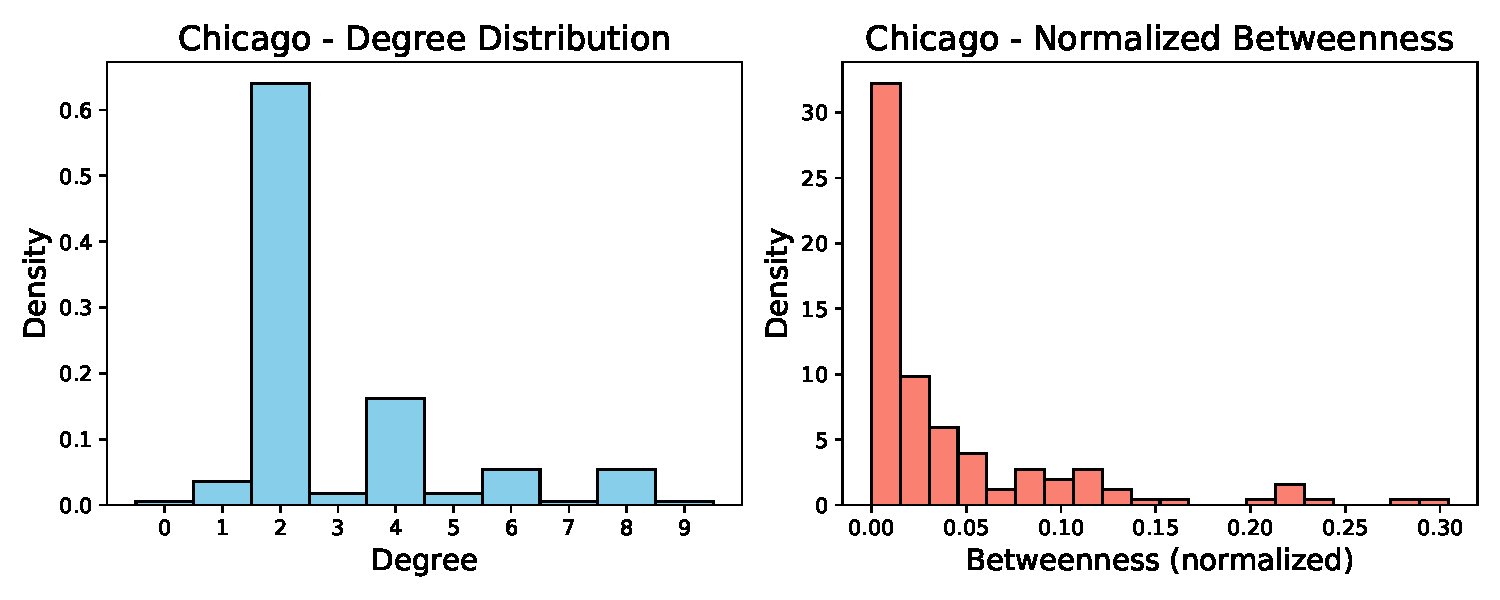
\includegraphics[width=\linewidth]{task40_plots/deg_bet_Chicago.pdf}
    \end{minipage}
\end{figure}

\begin{figure}[hbtp]
    \centering
    \begin{minipage}{0.48\linewidth}
        \centering
        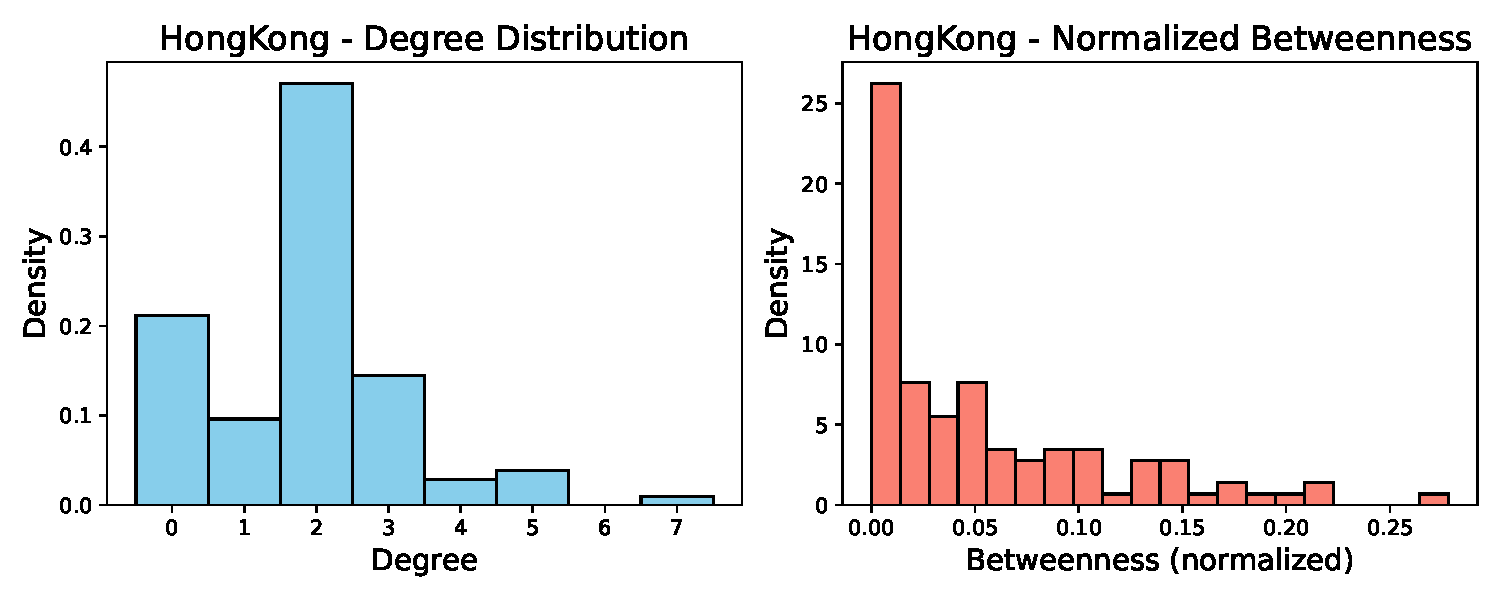
\includegraphics[width=\linewidth]{task40_plots/deg_bet_HongKong.pdf}
        \end{minipage}%
    \hfill
    \begin{minipage}{0.48\linewidth}
        \centering
        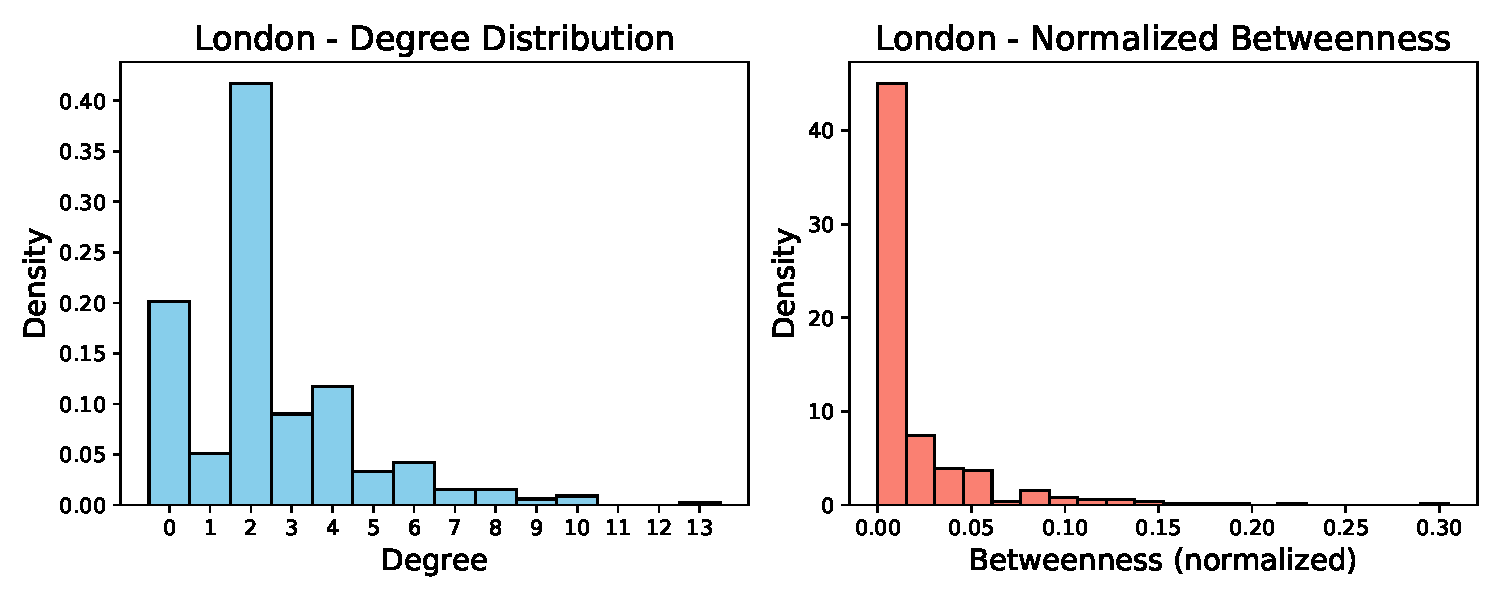
\includegraphics[width=\linewidth]{task40_plots/deg_bet_London.pdf}
    \end{minipage}
\end{figure}

\begin{figure}[h!]
    \centering
    \begin{minipage}{0.48\linewidth}
        \centering
        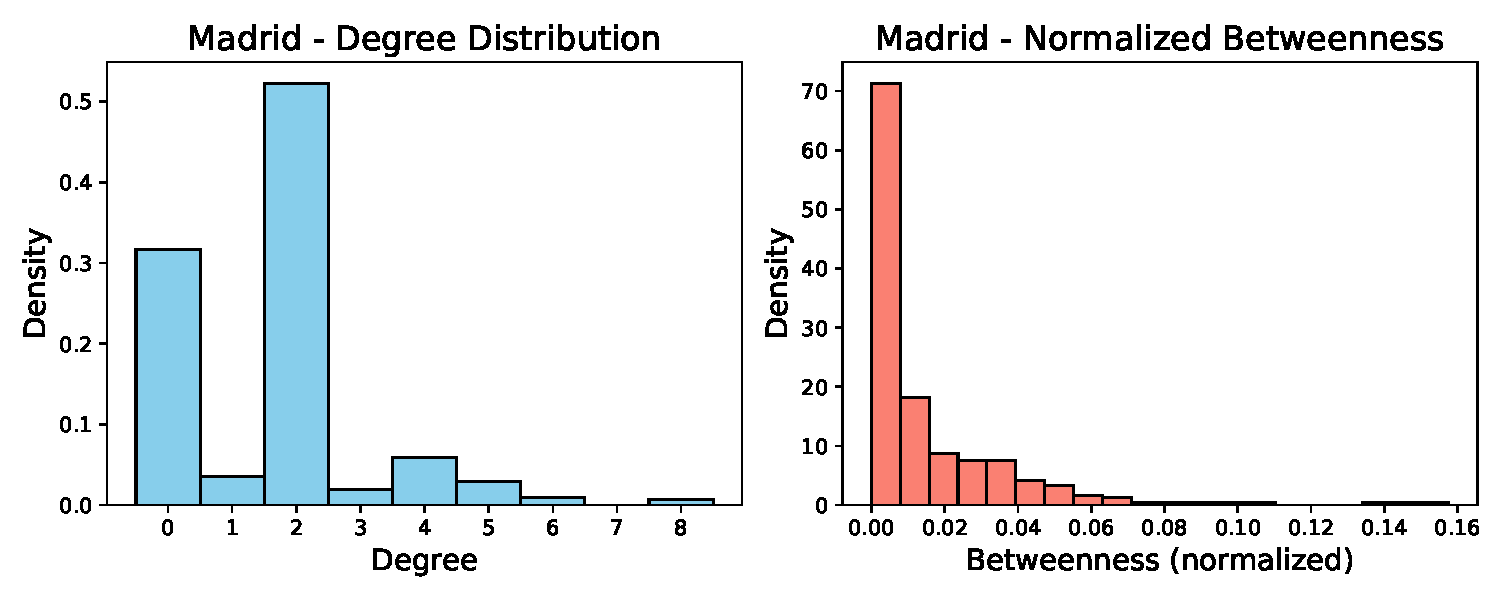
\includegraphics[width=\linewidth]{task40_plots/deg_bet_Madrid.pdf}
        \end{minipage}%
    \hfill
    \begin{minipage}{0.48\linewidth}
        \centering
        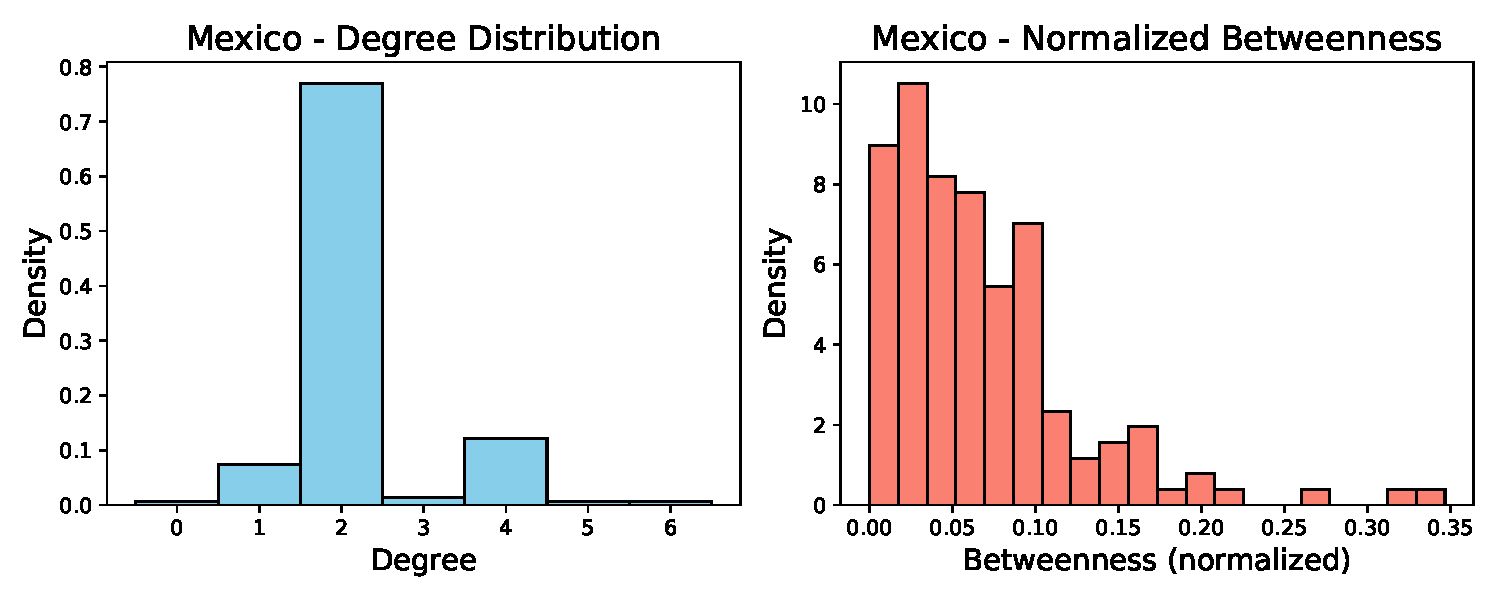
\includegraphics[width=\linewidth]{task40_plots/deg_bet_Mexico.pdf}
    \end{minipage}
\end{figure}

We further investigate the network’s structural characteristics by analyzing the average degree, assortativity, and shortest path length across nodes, providing insights into centrality patterns, degree correlations, and network compactness.

\begin{figure}[h!]
    \centering
    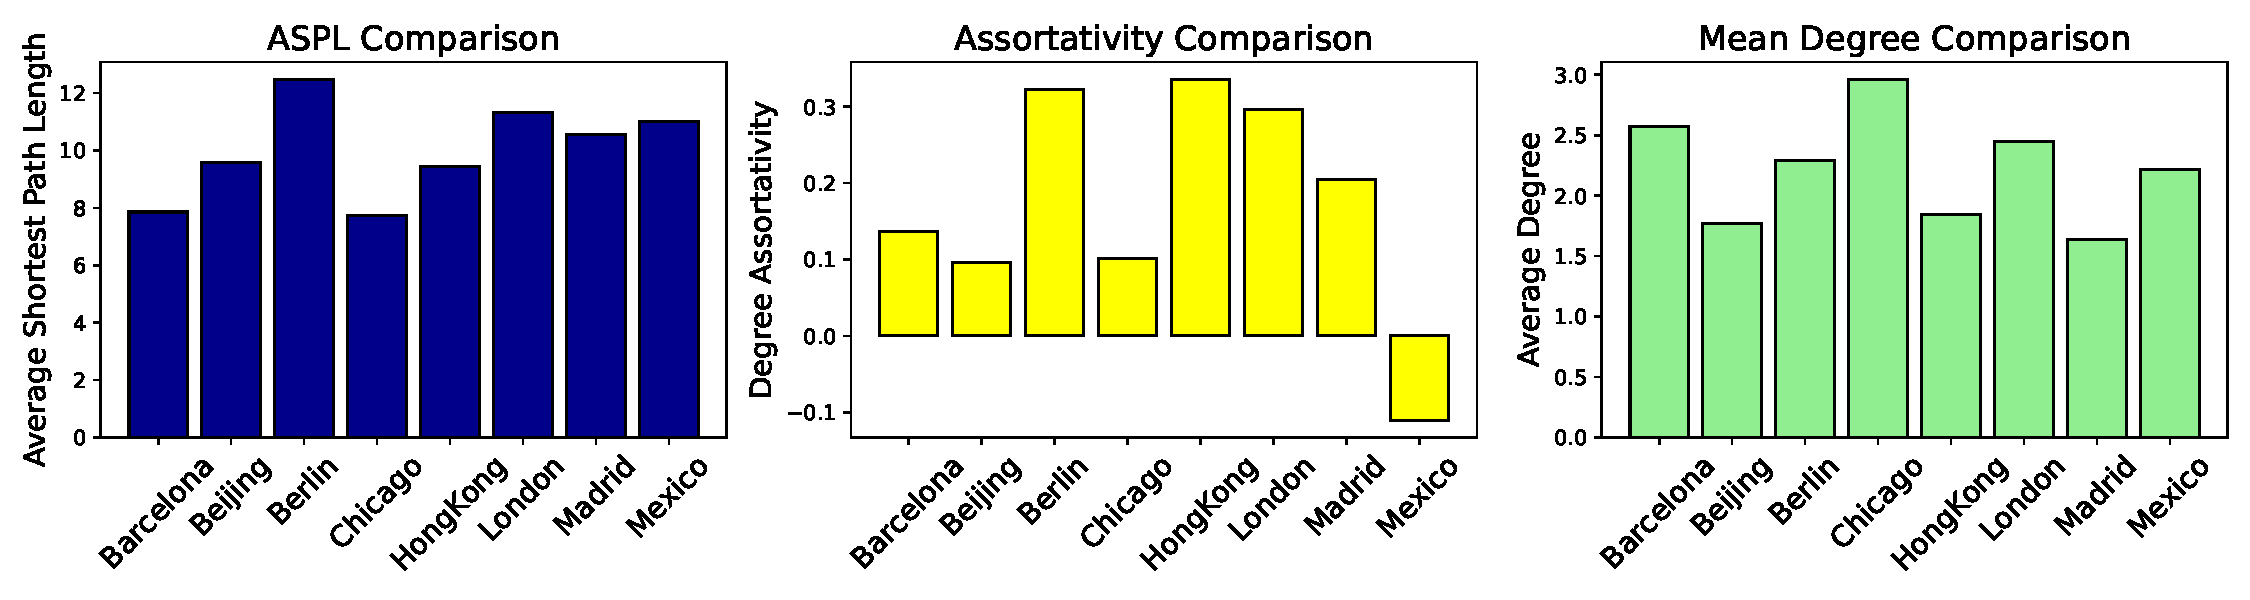
\includegraphics[width=0.70\linewidth]{task40_plots/comparison_plot.pdf}
    \caption{Comparison plot of some network's characteristics.}
    \label{fig:comparison_plot}
\end{figure}